\documentclass[unicode,11pt,a4paper,oneside,numbers=endperiod,openany]{scrartcl}

\renewcommand{\thesubsection}{\arabic{subsection}}

\usepackage{ifthen}
\usepackage[utf8]{inputenc}
\usepackage{graphics}
\usepackage{graphicx}
\usepackage{hyperref}

\pagestyle{plain}
\voffset -5mm
\oddsidemargin  0mm
\evensidemargin -11mm
\marginparwidth 2cm
\marginparsep 0pt
\topmargin 0mm
\headheight 0pt
\headsep 0pt
\topskip 0pt        
\textheight 255mm
\textwidth 165mm

\newcommand{\duedate} {}
\newcommand{\setduedate}[1]{%
\renewcommand\duedate {\textbf{Due date:}~ #1}}
\newcommand\isassignment {false}
\newcommand{\setassignment}{\renewcommand\isassignment {true}}
\newcommand{\ifassignment}[1]{\ifthenelse{\boolean{\isassignment}}{#1}{}}
\newcommand{\ifnotassignment}[1]{\ifthenelse{\boolean{\isassignment}}{}{#1}}

\newcommand{\assignmentpolicy}{
\begin{table}[h]
\begin{center}
\scalebox{0.8} {%
\begin{tabular}{|p{0.02cm}p{16cm}|}
\hline
&\\
\multicolumn{2}{|c|}{\Large\textbf{Numerical Computing 2023 ---  Submission Instructions}}\\
\multicolumn{2}{|c|}{\large\textbf{(Please, notice that following instructions are mandatory: }}\\
\multicolumn{2}{|c|}{\large\textbf{submissions that don't comply with, won't be considered)}}\\
&\\
\textbullet & Assignments must be submitted to \href{https://www.icorsi.ch/course/view.php?id=14666}{iCorsi} (i.e. in electronic format).\\
\textbullet & Provide both executable package and sources (e.g. C/C++ files, MATLAB). 
If you are using libraries, please add them in the file. Sources must be organized in directories called:\\
\multicolumn{2}{|c|}{\textit{Project\_number\_lastname\_firstname}}\\
& and  the  file must be called:\\
\multicolumn{2}{|c|}{\textit{project\_number\_lastname\_firstname.zip}}\\
\multicolumn{2}{|c|}{\textit{project\_number\_lastname\_firstname.pdf}}\\
\textbullet &  The TAs will grade your project by reviewing your project write-up, and looking at the implementation you attempted, and benchmarking your code's performance.\\

\textbullet & You are allowed to discuss all questions with anyone you like; however: (i) your submission must list anyone you discussed problems with and (ii) you must write up your submission independently.\\
\hline
\end{tabular}
}
\end{center}
\end{table}
}
\newcommand{\punkte}[1]{\hspace{1ex}\emph{\mdseries\hfill(#1~\ifcase#1{Points}\or{Points}\else{Points}\fi)}}


\newcommand\serieheader[6]{
\thispagestyle{empty}%
\begin{flushleft}

\includegraphics[width=0.45\textwidth]{CI_logo}
\end{flushleft}
  \noindent%
  {\large\ignorespaces{\textbf{#1}}\hspace{\fill}\ignorespaces{ \textbf{#2}}}\\ \\%
  {\large\ignorespaces #3 \hspace{\fill}\ignorespaces #4}\\
  \noindent%
  \bigskip
  \hrule\par\bigskip\noindent%
  \bigskip {\ignorespaces {\Large{\textbf{#5}}}
  \hspace{\fill}\ignorespaces \large \ifthenelse{\boolean{\isassignment}}{\duedate}{#6}}
  \hrule\par\bigskip\noindent%  \linebreak
 }

\makeatletter
\def\enumerateMod{\ifnum \@enumdepth >3 \@toodeep\else
      \advance\@enumdepth \@ne
      \edef\@enumctr{enum\romannumeral\the\@enumdepth}\list
      {\csname label\@enumctr\endcsname}{\usecounter
        {\@enumctr}%%%? the following differs from "enumerate"
	\topsep0pt%
	\partopsep0pt%
	\itemsep0pt%
	\def\makelabel##1{\hss\llap{##1}}}\fi}
\let\endenumerateMod =\endlist
\makeatother




\usepackage{textcomp}







\usepackage{float}
\usepackage{color}
\usepackage{listings}
\definecolor{mygreen}{rgb}{0,0.6,0}
\definecolor{mygray}{rgb}{0.5,0.5,0.5}
\definecolor{mymauve}{rgb}{0.58,0,0.82}

\lstset{ %
  backgroundcolor=\color{white},   % choose the background color
  basicstyle=\footnotesize,        % size of fonts used for the code
  breaklines=true,                 % automatic line breaking only at whitespace
  captionpos=b,                    % sets the caption-position to bottom
  commentstyle=\color{mygreen},    % comment style
  escapeinside={\%*}{*)},          % if you want to add LaTeX within your code
  keywordstyle=\color{blue},       % keyword style
  stringstyle=\color{mymauve},     % string literal style
  language=Matlab,                 % set MATLAB as the language
}



\begin{document}


\setassignment
\setduedate{Friday, December 29, 2023, 11:59 PM}

\serieheader{Numerical Computing}{2023}{Student: Harkeerat Singh Sawhney}{}{Solution for Project 5}{}
\newline

\assignmentpolicy

\newpage

\section{Graphical Solution of Linear Programming Problems [20 points]}
\subsection{Problem 1}
\subsubsection{Solve the System of Inequalities}
We are asked to solve the system of inequalities, which is already given in the question itself.

\begin{equation}
	\begin{aligned}
		min \quad  & z = 4x + y      \\
		s.t. \quad & x + 2y \leq 40  \\
		           & x + y \geq 30   \\
		           & 2x + 3y \geq 72 \\
		           & x, y \geq 0
	\end{aligned}
	\label{eq:1.1.1}
\end{equation}

Hence as it can be seen from the Equation \ref{eq:1.1.1}, we have to find the minimum value of $z$ such that the constraints are satisfied. This can be solved graphically by plotting the constraints and finding the minimum value of $z$. Before that lets rewrite the constraints in the form of $y = mx + c$ which can be seen at Equation \ref{eq:1.1.2}.

\begin{equation}
	\begin{aligned}
		min \quad  & z = 4x + y             \\
		s.t. \quad & y = -\frac{1}{2}x + 20 \\
		           & y = -x + 30            \\
		           & y = -\frac{2}{3}x + 24 \\
		           & x, y \geq 0
	\end{aligned}
	\label{eq:1.1.2}
\end{equation}

\subsubsection{Plot the feasible region identified by the constraints.}

\begin{figure}[H]
	\centering
	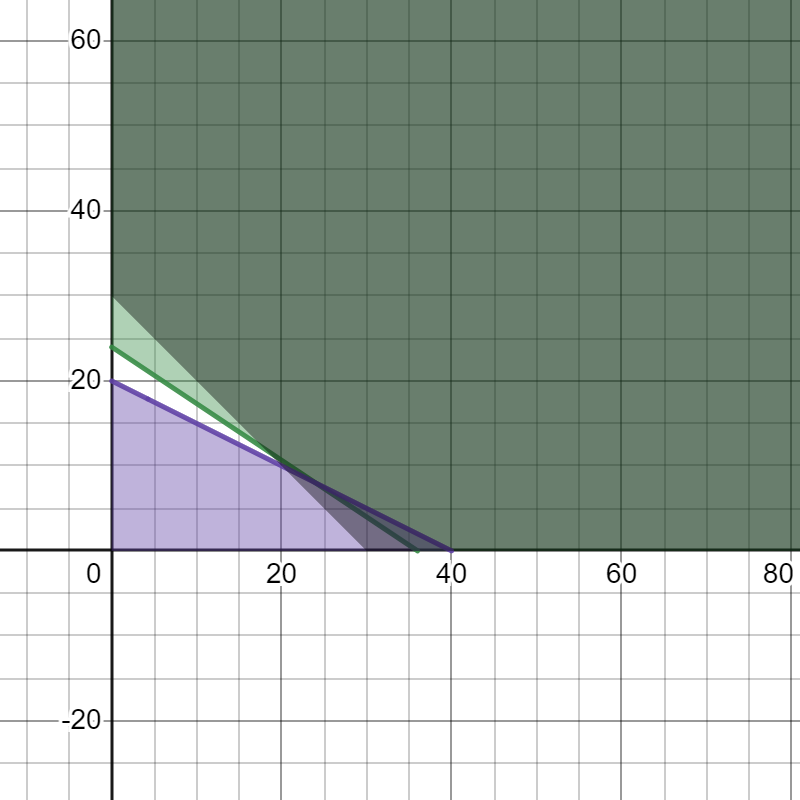
\includegraphics[width=0.5\linewidth]{figures/problem_1.1.1.png}
	\caption{Plot of all the constraints for Problem 1}
	\label{fig:problem_1.1}
\end{figure}
Now we can plot the constraints on a graph as shown in Figure \ref{fig:problem_1.1}. Figure \ref{fig:problem_1.1} is showing the plot of all the constraints. All of these constraints can be seen by their respective colors. However what we are interested is in the region where all the constraints maximum, as that region would include all minimum value of $z$.

\begin{figure}[H]
	\centering
	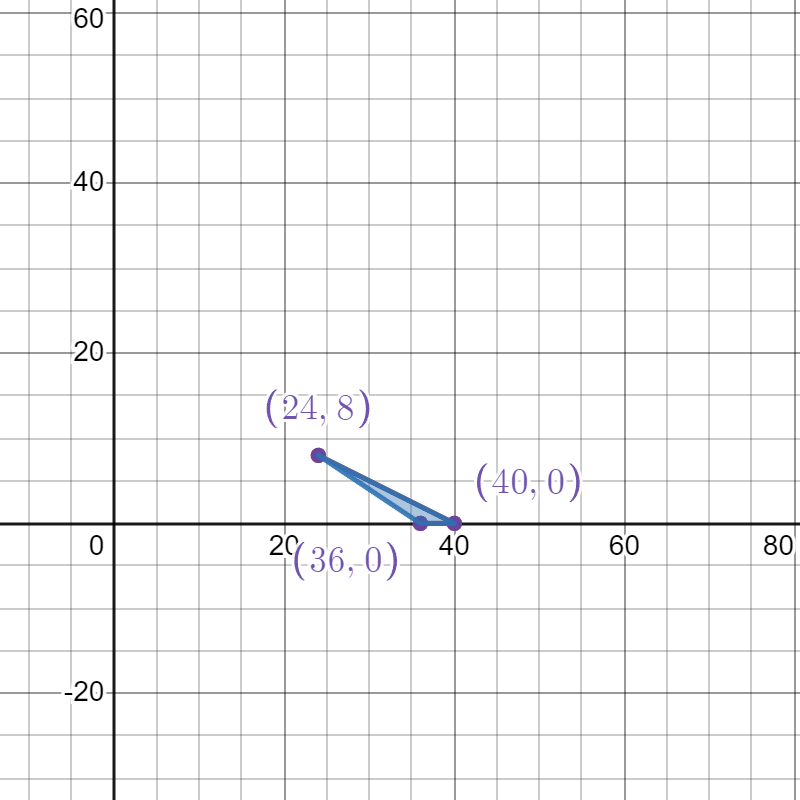
\includegraphics[width=0.5\linewidth]{figures/problem_1.1.2.png}
	\caption{Shading the region where all the constraints maximum for Problem 1}
	\label{fig:problem_1.2}
\end{figure}

As it can be seen from the Figure \ref{fig:problem_1.2}, the region where all the constraints maximum is the region where the minimum value of $z$ would be. Here what is important for us is the points of intersection of the constrains with each other and the points of intersection of the constraints with the axes. These points are as well shown in the Figure \ref{fig:problem_1.2}. These points are as follows:

\begin{itemize}
	\item $(24, 8)$
	\item $(40, 0)$
	\item $(36, 0)$
\end{itemize}

\subsubsection{ Find the optimal solution and the value of the objective function in that point.}
Now from the previous part we have the points of intersection of the constraints with each other and the points of intersection of the constraints with the axes. What we need to do now is to find the minium value of $z$ at these points. Hence we have to evaluate the objective function at each vertices and pick the minimum value of $z$. The vertices are as follows:

\begin{equation}
	\begin{aligned}
		At \quad (24, 8) \quad z = 4(24) + 8 = 104 \\
		At \quad (40, 0) \quad z = 4(40) + 0 = 160 \\
		At \quad (36, 0) \quad z = 4(36) + 0 = 144
	\end{aligned}
	\label{eq:1.1.3}
\end{equation}

From the Equation \ref{eq:1.1.3} we can see that the minimum value of $z$ is at $(24, 8)$ which is $104$.

\subsection{Problem 2}
\subsubsection{Solve the System of Inequalities}
This is a bit more tricker than the previous problem, as unlike previous problem we do now have the mathematical form of the constraints. We have a real life problem from which we have to convert to the mathematical form. The problem is as follows:

\begin{quote}
	\textit{A tailor plans to sell two types of trousers, with production costs of $25 $ CHF and $40$ CHF, respectively. The former type can be sold for $85$ CHF, while the latter for $110$ CHF. The tailor estimates a total monthly demand of $265$ trousers. Find the number of units of each type of trousers that should be produced in order to maximize the net profit of the tailor, if we assume that the he cannot spend more than $7000$ CHF in raw materials.?}
\end{quote}

Hence from the above problem we can see that we have to find the maximum value of $z$ which is the net profit of the tailer. The variables are as follows:


\begin{itemize}
	\item $x$ = Number of trousers of type 1
	\item $y$ = Number of trousers of type 2
	\item $z$ = Net profit of the tailor
\end{itemize}

We have obtained the Objective Function (Maximize Profit $z$) by knowing that the profit from selling the first type of trousers is $85 - 25 = 60$ CHF and the profit from selling the second type of trousers is $110 - 40 = 70$ CHF. Hence we can write the Objective Function as follows:

\begin{equation}
	\begin{aligned}
		Maximize \quad & z = 60x + 70y \\
	\end{aligned}
	\label{eq:1.1.4}
\end{equation}

We know that the total demand of trousers is $265$ and the total amount of money that can be spent on raw materials is $7000$ CHF. Hence we can write the first constraint as follows:

\begin{equation}
	\begin{aligned}
		x + y \leq 265 \\
	\end{aligned}
	\label{eq:1.1.5}
\end{equation}

We also know that the cost of producing the first type of trousers is $25$ CHF and the cost of producing the second type of trousers is $40$ CHF. Hence we can write the second constraint as follows:

\begin{equation}
	\begin{aligned}
		25x + 40y \leq 7000 \\
	\end{aligned}
	\label{eq:1.1.6}
\end{equation}

Hence finally by combining the Equation \ref{eq:1.1.4}, \ref{eq:1.1.5} and \ref{eq:1.1.6} we can write the constraints as follows in the mathematical form at Equation \ref{eq:1.1.7}.

\begin{equation}
	\begin{aligned}
		min \quad  & z = 60x + 25y       \\
		s.t. \quad & x + y \leq 265      \\
		           & 25x + 40y \leq 7000 \\
		           & x, y \geq 0
	\end{aligned}
	\label{eq:1.1.7}
\end{equation}

Now we must rewrite the constraints in the form of $y = mx + c$ which can be seen at Equation \ref{eq:1.1.8}.

\begin{equation}
	\begin{aligned}
		min \quad  & z = 60x + 25y           \\
		s.t. \quad & y = -x + 265            \\
		           & y = -\frac{5}{8}x + 175 \\
		           & x, y \geq 0
	\end{aligned}
	\label{eq:1.1.8}
\end{equation}

\subsubsection{Plot the feasible region identified by the constraints.}

\begin{figure}[H]
	\centering
	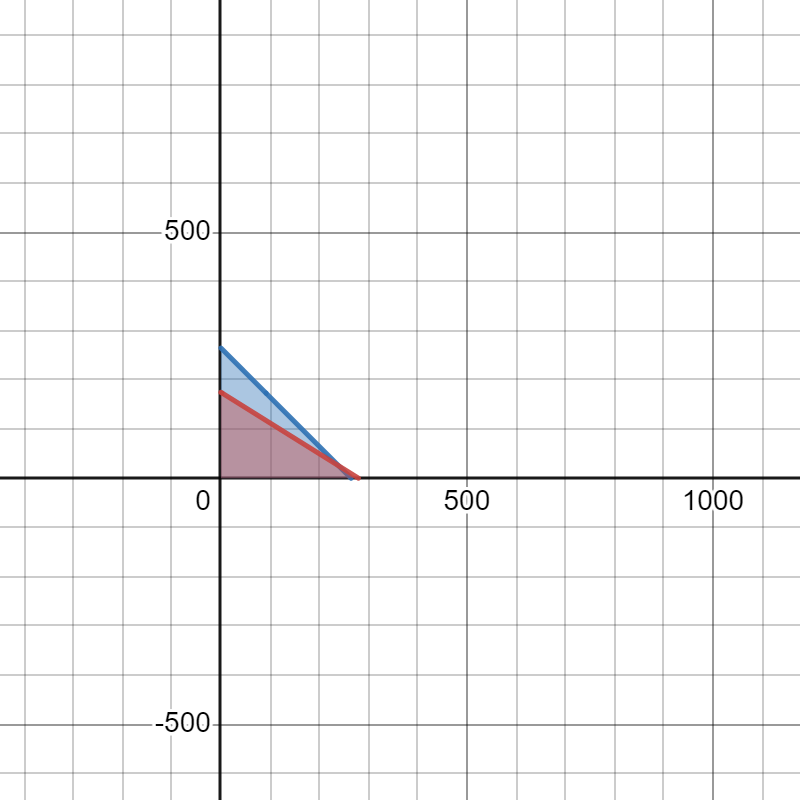
\includegraphics[width=0.5\linewidth]{figures/problem_1.2.1.png}
	\caption{Plot of all the constraints for Problem 2}
	\label{fig:problem_2.1}
\end{figure}

Again very similar to the previous problem, we have to plot the constraints on a graph as shown in Figure \ref{fig:problem_2.1}. Figure \ref{fig:problem_2.1} is showing the plot of all the constraints and all of these constraints can be seen by their respective colors. However what we are interested is in the region where all the constraints maximum, as that region would include all maximize value of $z$.

\begin{figure}[H]
	\centering
	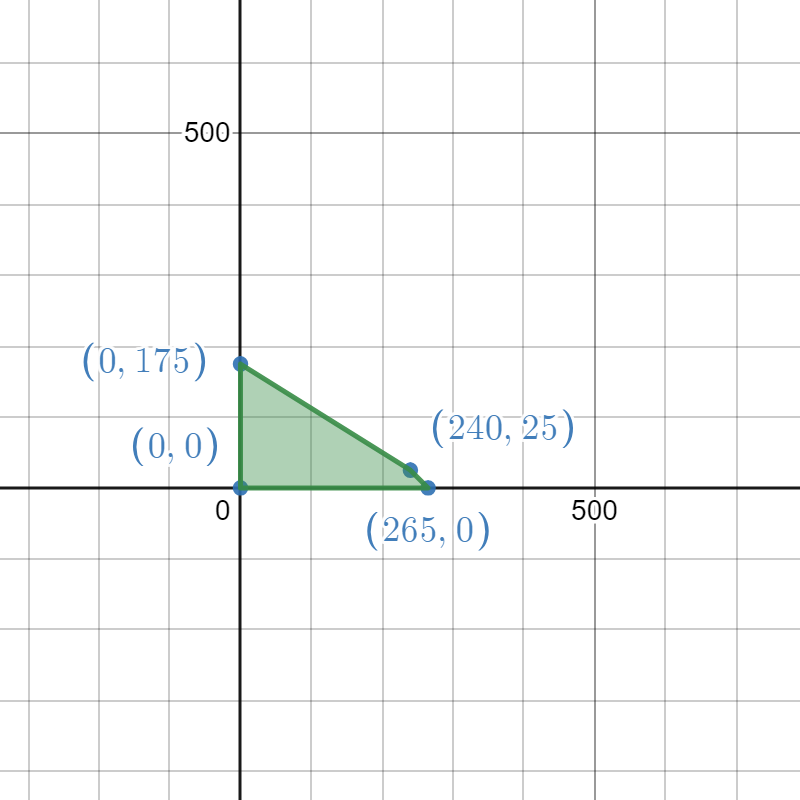
\includegraphics[width=0.5\linewidth]{figures/problem_1.2.2.png}
	\caption{Shading the region where all the constraints maximum for Problem 2}
	\label{fig:problem_2.2}
\end{figure}

As it can be seen from the Figure \ref{fig:problem_2.2}, the region where all the constraints maximum is the region where the maximum value of $z$ would be. Here what is important for us is the points of intersection of the constrains with each other and the points of intersection of the constraints with the axes. These points are as well shown in the Figure \ref{fig:problem_2.2}. These points are as follows:

\begin{itemize}
	\item $(0, 175)$
	\item $(240, 25)$
	\item $(265, 0)$
	\item $(0, 0)$
\end{itemize}

\subsubsection{ Find the optimal solution and the value of the objective function in that point.}

Now from the previous part we have the points of intersection of the constraints with each other and the points of intersection of the constraints with the axes. What we need to do now is to find the minium value of $z$ at these points. Hence we have to evaluate the objective function at each vertices and pick the minimum value of $z$. The vertices are as follows:

\begin{equation}
	\begin{aligned}
		At \quad (0, 175) \quad z = 60(0) + 25(175) = 4375    \\
		At \quad (240, 25) \quad z = 60(240) + 25(25) = 15025 \\
		At \quad (265, 0) \quad z = 60(265) + 25(0) = 15900   \\
		At \quad (0, 0) \quad z = 60(0) + 25(0) = 0
	\end{aligned}
	\label{eq:1.1.9}
\end{equation}

From the Equation \ref{eq:1.1.9} we can see that the maximum value of $z$ is at $(265, 0)$ which is $15900$.

\section{Implementation of the Simplex Method [30 points]}
In this question we are asked to implement the Simplex Method for the Linear Programming Problem. We are asked to complete the 2 functions which are as follows:

\begin{itemize}
	\item \texttt{standardise.m}
	\item \texttt{simplexSolve.m}
\end{itemize}

Before explaining the implementation of the functions, I will first explain how the Simplex Method works. The Simplex Method is an iterative method for solving the Linear Programming Problems, in which it first starts with a feasible solution and then iteratively improves the solution until the optimal solution is reached. This is what the Matlab implementation of the Simplex Method is doing as well. 

\subsection{standardise.m}
This function is used to standardize the Linear Programming Problem which is used to a form which can be used by other methods. This functions takes in total 6 arguments which are as follows:

\begin{itemize}
	\item \texttt{type} = A string which tells whether the problem is a maximization or minimization problem
	\item \texttt{A} = A matrix of the coefficients of the constraints
	\item \texttt{h} = The right hand side of the constraints
	\item \texttt{c} = The coefficients of the objective function
	\item \texttt{m} = The number of constraints
	\item \texttt{sign} = A vector indicating the sign of the constraints
\end{itemize}

\subsubsection{Summery of the function}
The function first initializes an identity matrix of size $m \times m$. Then it checks if the problem is a maximization or minimization problem. If the problem is a maximization problem then it uses the surplus variables (changes the sign of the corresponding row in the identity matrix), however if it is a minimization problem then it uses the slack variables (does not change the sign of the corresponding row in the identity matrix).

The next step is to ensure that all the values in the right-hand side ($h$) are positive. If any of the values are negative then it changes the sign of the corresponding row in $A, h$ and the augmented matrix. This is done because the Simplex Method only works for the problems where the right-hand side is positive. This was the To-Do which we were supposed to implement, which was done by creating a for-loop which checks if any of the values in $h$ is less than $0$ and if it is, it multiplies the corresponding row in $A, h$ and the augmented matrix by $-1$. After that the functions arguments are returned.

\subsection{simplexSolve.m}
This function takes the following arguments:

\begin{itemize}
	\item \texttt{type} = A string which tells whether the problem is a maximization or minimization problem
	\item \texttt{A} = A matrix of the coefficients of the constraints
	\item \texttt{h} = The right hand side of the constraints
	\item \texttt{c} = The coefficients of the objective function
	\item \texttt{sign} = A vector indicating the sign of the constraints
\end{itemize}

What this functions is supposed to do is to standardize the problem using the standardize function (which was explained in the previous section) and then determine a optimal starting solution which uses auxiliary function. Finally it solves the linear programming problem using the simplexSolve function and computes the value of the objective function at the optimal solution.

\subsubsection{Summery of the function}
First the function calculates the number of constraints $m$ and the number of variables $n$ from the dimensions of $A$. It also calculates the $itMax$ which is the maximum number of iteration which the Simplex Method can do. This was done by using taking in the number of constraints and the number of variables and then multiplying them by $2$. This was done because the maximum number of iterations which the Simplex Method can do is $(m + n) \space chose \space m$. In the actual code (which we were supposed to implement) we first calculated the factorial of $(m + n)$ and then divided it by the factorial of $m$ and factorial of $n$. With this we calculated the binomial coefficient of $(m + n) \space chose \space m$.

After this it computes the standard form of the problem using the standardize function. Then it determines a starting solution using the auxiliary function. Finally it solves the linear programming problem using the simplexSolve function and computes the value of the objective function at the optimal solution. After that it computes the value of the function by multiplying the coefficient of the objective function with the optimal solution. Finally it returns the optimal solution and the value of the objective function.

\subsection{simplexSolve.m}

This function has the implementation of the Simplex Method. It first initializes the number of iteration $nIter$ to $0$. It as well computes the $BB^{-1}*D$ and $B^{-1}*h$, which are the initial values of the Simplex Method. After this it computes the reduce coefficients (which we were supposed to implement). This was done by using the formula $r\_d = c\_d - c\_B * (B \backslash D)$ THese coefficients are used to determine which of these variables should be added to the basis. Then this function checks if it is an optimal solution or not. If it is a maximization problem, then the solution would be optimal if all the reduce cost coefficients are non-positive. However, if it is a minimization problem, the solution is optimal if all reduced cost coefficients are non-positive. 

Now the main loop is formulated which keeps on going until the optimal condition is satisfied. In the loop the following is done in each iteration:

\begin{itemize}
	\item Entering the Variable: If it is a maximization problem the variable with the largest positive reduced cost coefficient enters the basis. If it is a minimization problem., the variable with the smallest negative reduced cost coefficient enters the basis.
	\item Evaluation of the coefficient ratios: The variable is determined which would leave the basis. This is done by computing the coefficient ratios $B^{-1}*h$ to $B^{-1}$ in for each basic variable and then it choses the variable with the smallest positive ratio.
	\item Update the Matrices: The matrices $B$, $D$, cost vectors and the indices are updated by swapping the entering and leaving variables.
	\item Recomputing the reduced cost coefficients: The reduced cost coefficients are recomputed using the formula $r\_d = c\_d - c\_B * (B \backslash D)$.
	\item Checking the optimality condition: The optimality condition is checked again and if it is satisfied then the loop is terminated.
	\item Checking the Loop bound: If the number of iterations exceeds the maximum number of iterations then the loop is terminated.
	\item Computing the optimal solution: The optimal solution is computed using the formula $x\_B = B \backslash h$.
\end{itemize}

Finally the optimal solution and the value of the objective function is returned.



At last we ran the \texttt{test\_simplexSolve.m} it has shown that all the tests have passed. Hence we can say that the implementation of the Simplex Method is correct.

\section{Applications to Real-Life Example: Cargo Aircraft [25 points]}
\subsection{Formulate the problem as a linear program: what is the objective function? What are the constraints?
	Write down all equations, with comments explaining what you are doing.}


In this Question we are asked to solve a real life Linear Programming Problem. The problem is that we have a cargo aircraft which has 4 components and we have to find the optimal way to load the cargo in the aircraft. Bellow is the table which shows the compartments and their capacities.

\begin{table}[H]
	\centering
	\begin{tabular}{|c|c|c|}
		\hline
		Compartment & Weight Capacity (t) & Storage Capacity (m3) \\
		\hline
		S1          & 18                  & 11930                 \\
		S2          & 32                  & 22552                 \\
		S3          & 25                  & 11209                 \\
		S4          & 17                  & 5870                  \\
		\hline
	\end{tabular}
	\caption{Compartments and their capacities}
	\label{tab:2.1}
\end{table}

\begin{table}[H]
	\centering
	\begin{tabular}{|c|c|c|c|}
		\hline
		Cargo & Weight (t) & Volume (m3/t) & Profit (CHF/t) \\
		\hline
		C1    & 16         & 320           & 135            \\
		C2    & 32         & 510           & 200            \\
		C3    & 40         & 630           & 410            \\
		C4    & 28         & 125           & 520            \\
		\hline
	\end{tabular}
	\caption{Cargos and their properties}
	\label{tab:2.2}
\end{table}

As it can be seen in the Table \ref{tab:2.1} and \ref{tab:2.2} that we have 4 compartments and 4 cargos. The compartments have their weight capacity and storage capacity. The cargos have their weight, volume and profit. Along with that we also know that the profit obtained for each cargo increases by some percentage depending on the compartment in which it is stored. This percentage is as follows:

\begin{itemize}
	\item $S1$ = $0\%$
	\item $S2$ = $10\%$
	\item $S3$ = $20\%$
	\item $S4$ = $30\%$
\end{itemize}

\subsubsection{Objective Function}
The objective function is to maximize the profit. The profit is obtained by multiplying the profit of each cargo with the percentage increase in the profit depending on the compartment in which it is stored. hence the objective function is as follows:

Lets first define the variables which we are going to use in the objective function. $x_{ij}$ is the number of cargos of type $i$ stored in compartment $j$. So for example $x_{11}$ is the number of cargos of type $1$ stored in compartment $1$. 

\textbf{Objective Function}

\begin{equation}
	\begin{aligned}
		Maximize \quad & z = 135 \times 1 \times \sum_{j=1}^{4} x_{1j} + 200 \times 1.1 \times \sum_{j=1}^{4} x_{2j} + 410 \times 1.2 \times \sum_{j=1}^{4} x_{3j} + 520 \times 1.3 \times \sum_{j=1}^{4} x_{4j} \\
	\end{aligned}
	\label{eq:2.1.1}
\end{equation}

\subsubsection{Constraints}
The objective function is to maximize the profit. However we have some constraints which we have to follow in order to maximize the profit. These constraints are as follows:

\begin{itemize}
	\item The weight of the cargo in each compartment should not exceed the weight capacity of the compartment.
	\item The volume of the cargo in each compartment should not exceed the volume capacity of the compartment.
	\item The total number of cargos of each type should not exceed the total number of cargos available.
	\item We need to follow the non-negativity constraint.
\end{itemize}

Bellow is the visualization of the constraints:

\textbf{Weight Constraint}
\begin{equation}
	\begin{aligned}
		x_{11} + x_{12} + x_{13} + x_{14} \leq 18 \\
		x_{21} + x_{22} + x_{23} + x_{24} \leq 32 \\
		x_{31} + x_{32} + x_{33} + x_{34} \leq 25 \\
		x_{41} + x_{42} + x_{43} + x_{44} \leq 17 \\
	\end{aligned}
	\label{eq:2.1.2}
\end{equation}

\textbf{Volume Constraint}
\begin{equation}
	\begin{aligned}
		320x_{11} + 510x_{12} + 630x_{13} + 125x_{14} \leq 11930 \\
		320x_{21} + 510x_{22} + 630x_{23} + 125x_{24} \leq 22552 \\
		320x_{31} + 510x_{32} + 630x_{33} + 125x_{34} \leq 11209 \\
		320x_{41} + 510x_{42} + 630x_{43} + 125x_{44} \leq 5870  \\
	\end{aligned}
	\label{eq:2.1.3}
\end{equation}

\textbf{Number of Cargos Constraint}
\begin{equation}
	\begin{aligned}
		x_{11} + x_{12} + x_{13} + x_{14} \leq 16 \\
		x_{21} + x_{22} + x_{23} + x_{24} \leq 32 \\
		x_{31} + x_{32} + x_{33} + x_{34} \leq 40 \\
		x_{41} + x_{42} + x_{43} + x_{44} \leq 28 \\
	\end{aligned}
	\label{eq:2.1.4}
\end{equation}

\textbf{Non-Negativity Constraint}
\begin{equation}
	\begin{aligned}
		x_{ij} \geq 0 \quad \forall i, j
	\end{aligned}
	\label{eq:2.1.5}
\end{equation}

\subsection{Create a script \texttt{exercise2.m} which uses the simplex method implemented in the previous exercise to solve the problem. What is the optimal solution? Visualize it graphically and briefly comment the results obtained (are you surprised of this outcome on the basis of your data?).}

By using the \texttt{simplexSolve.m} function which we implemented in the previous exercise, we can solve the problem. The code for the \texttt{exercise2.m} is as follows:



\begin{lstlisting}
	type = 'max';

	A = [1,0,0,0, 1,0,0,0 ,1,0,0,0 ,1,0,0,0;
		0,1,0,0 ,0,1,0,0 ,0,1,0,0 ,0,1,0,0;
		0,0,1,0 ,0,0,1,0 ,0,0,1,0 ,0,0,1,0;
		0,0,0,1 ,0,0,0,1 ,0,0,0,1 ,0,0,0,1;
		320,0,0,0 ,510,0,0,0 ,630,0,0,0 ,125,0,0,0;
		0,320,0,0 ,0,510,0,0 ,0,630,0,0 ,0,125,0,0;
		0,0,320,0 ,0,0,510,0 ,0,0,630,0 ,0,0,125,0;
		0,0,0,320 ,0,0,0,510 ,0,0,0,630 ,0,0,0,125;
		1,1,1,1 ,0,0,0,0 ,0,0,0,0 ,0,0,0,0;
		0,0,0,0 ,1,1,1,1 ,0,0,0,0 ,0,0,0,0;
		0,0,0,0 ,0,0,0,0 ,1,1,1,1 ,0,0,0,0;
		0,0,0,0 ,0,0,0,0 ,0,0,0,0 ,1,1,1,1;];



	h = [18; 32; 25; 17; 11930; 22552; 11209; 5870; 16; 32; 40; 28];

	c = [135, 135*1.1, 135*1.2, 135*1.3, 200, 200*1.1, 200*1.2, 200*1.3, 410, 410*1.1, 410*1.2, 410*1.3, 520, 520*1.1, 520*1.2, 520*1.3];

	sign = [0, 0, 0, 0, 0, 0, 0, 0, 0, 0, 0, 0];


	[z, x_B, index_B] = simplex(type, A, h, c, sign);
	fprintf('z = %d\n', z);
	fprintf('x_B = \n');
	disp(x_B);
	fprintf('index_B = \n');
	disp(index_B);

	bar(x_B);
	title('Solution (x_B)');
	xlabel('Index');
	ylabel('Value');
\end{lstlisting}
\label{code:2.2.1}

As it can be seen from the code \ref{code:2.2.1}, we have used the \texttt{simplexSolve.m} function to solve the problem. However the trick part for this question was to formulate the problem in the form which can be used by the \texttt{simplexSolve.m} function. We first created the variable $A$ which is the matrix of the coefficients of the constraints. Then we created the variable $h$ which is the right hand side of the constraints. Then we created the variable $c$ which is the coefficients of the objective function. Finally we created the variable $sign$ which is a vector indicating the sign of the constraints.

After running the script the maximum profit which we can obtain is $z =  41890$. From the data I did not believe that the profit will be as high as that, as the profit for each cargo is not that high. However the profit is high because of the percentage increase in the profit depending on the compartment in which it is stored. Since we got the optimal solution, we maximized our profit from those percentage increase. 



\begin{figure}[H]
	\centering
	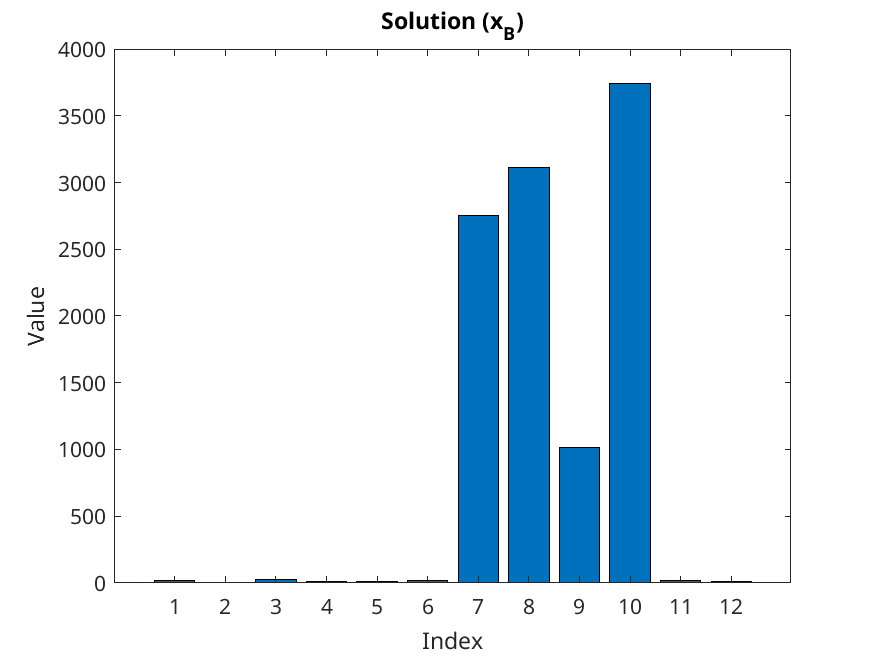
\includegraphics[width=0.5\linewidth]{figures/problem_2.png}
	\caption{Plot of the $x\_B$}
	\label{fig:problem_2}
\end{figure}

The Figure \ref{fig:problem_2} shows the plot of the $x\_B$. $x\_B$ is the vector which contains the basic variables.


\section{Cycling and Degeneracy [10 points]}
I tried to implement this problem in the similar way as the previous question, however I am getting the error of saying \texttt{Incorrect loop, more iterations than the number of basic solutions}. I tried to debug the code, however I was not able to find the error. Hence I am submitting the code which I have implemented. The code is as follows:

\begin{lstlisting}
	type = 'max';
	A = [4, 3; 4, 1; 4, 2;];
	h = [12; 8; 8];
	c = [3, 4];
	sign = [-1, -1, -1];

	[z, x_B, index_B] = simplex(type, A, h, c, sign);
\end{lstlisting}



\end{document}
